% Options for packages loaded elsewhere
\PassOptionsToPackage{unicode}{hyperref}
\PassOptionsToPackage{hyphens}{url}
\documentclass[
  ignorenonframetext,
]{beamer}
\newif\ifbibliography
\usepackage{pgfpages}
\setbeamertemplate{caption}[numbered]
\setbeamertemplate{caption label separator}{: }
\setbeamercolor{caption name}{fg=normal text.fg}
\beamertemplatenavigationsymbolsempty
% remove section numbering
\setbeamertemplate{part page}{
  \centering
  \begin{beamercolorbox}[sep=16pt,center]{part title}
    \usebeamerfont{part title}\insertpart\par
  \end{beamercolorbox}
}
\setbeamertemplate{section page}{
  \centering
  \begin{beamercolorbox}[sep=12pt,center]{section title}
    \usebeamerfont{section title}\insertsection\par
  \end{beamercolorbox}
}
\setbeamertemplate{subsection page}{
  \centering
  \begin{beamercolorbox}[sep=8pt,center]{subsection title}
    \usebeamerfont{subsection title}\insertsubsection\par
  \end{beamercolorbox}
}
% Prevent slide breaks in the middle of a paragraph
\widowpenalties 1 10000
\raggedbottom
\AtBeginPart{
  \frame{\partpage}
}
\AtBeginSection{
  \ifbibliography
  \else
    \frame{\sectionpage}
  \fi
}
\AtBeginSubsection{
  \frame{\subsectionpage}
}
\usepackage{iftex}
\ifPDFTeX
  \usepackage[T1]{fontenc}
  \usepackage[utf8]{inputenc}
  \usepackage{textcomp} % provide euro and other symbols
\else % if luatex or xetex
  \usepackage{unicode-math} % this also loads fontspec
  \defaultfontfeatures{Scale=MatchLowercase}
  \defaultfontfeatures[\rmfamily]{Ligatures=TeX,Scale=1}
\fi
\usepackage{lmodern}
\ifPDFTeX\else
  % xetex/luatex font selection
\fi
% Use upquote if available, for straight quotes in verbatim environments
\IfFileExists{upquote.sty}{\usepackage{upquote}}{}
\IfFileExists{microtype.sty}{% use microtype if available
  \usepackage[]{microtype}
  \UseMicrotypeSet[protrusion]{basicmath} % disable protrusion for tt fonts
}{}
\makeatletter
\@ifundefined{KOMAClassName}{% if non-KOMA class
  \IfFileExists{parskip.sty}{%
    \usepackage{parskip}
  }{% else
    \setlength{\parindent}{0pt}
    \setlength{\parskip}{6pt plus 2pt minus 1pt}}
}{% if KOMA class
  \KOMAoptions{parskip=half}}
\makeatother
\usepackage{longtable,booktabs,array}
\newcounter{none} % for unnumbered tables
\usepackage{calc} % for calculating minipage widths
\usepackage{caption}
% Make caption package work with longtable
\makeatletter
\def\fnum@table{\tablename~\thetable}
\makeatother
\setlength{\emergencystretch}{3em} % prevent overfull lines
\providecommand{\tightlist}{%
  \setlength{\itemsep}{0pt}\setlength{\parskip}{0pt}}
\usepackage{bookmark}
\IfFileExists{xurl.sty}{\usepackage{xurl}}{} % add URL line breaks if available
\urlstyle{same}
\hypersetup{
  hidelinks,
  pdfcreator={LaTeX via pandoc}}

\author{\texorpdfstring{}{}}
\date{}

\begin{document}

\begin{frame}{Security Implications}
\protect\phantomsection\label{sec:security}
The meta-level framework has significant implications for cognitive
security, AI safety, and the robustness of belief systems. Understanding
meta-cognitive processing reveals vulnerabilities that traditional
security models miss, while also suggesting principled defense
strategies.

\begin{block}{Cognitive Security Framework}
\protect\phantomsection\label{sec:cognitive_security_framework}
Active Inference's quadrant structure provides a systematic way to
analyze cognitive vulnerabilities. Each quadrant represents a potential
attack surface with distinct vulnerability profiles and defense
requirements.

\begin{figure}[h]
\centering
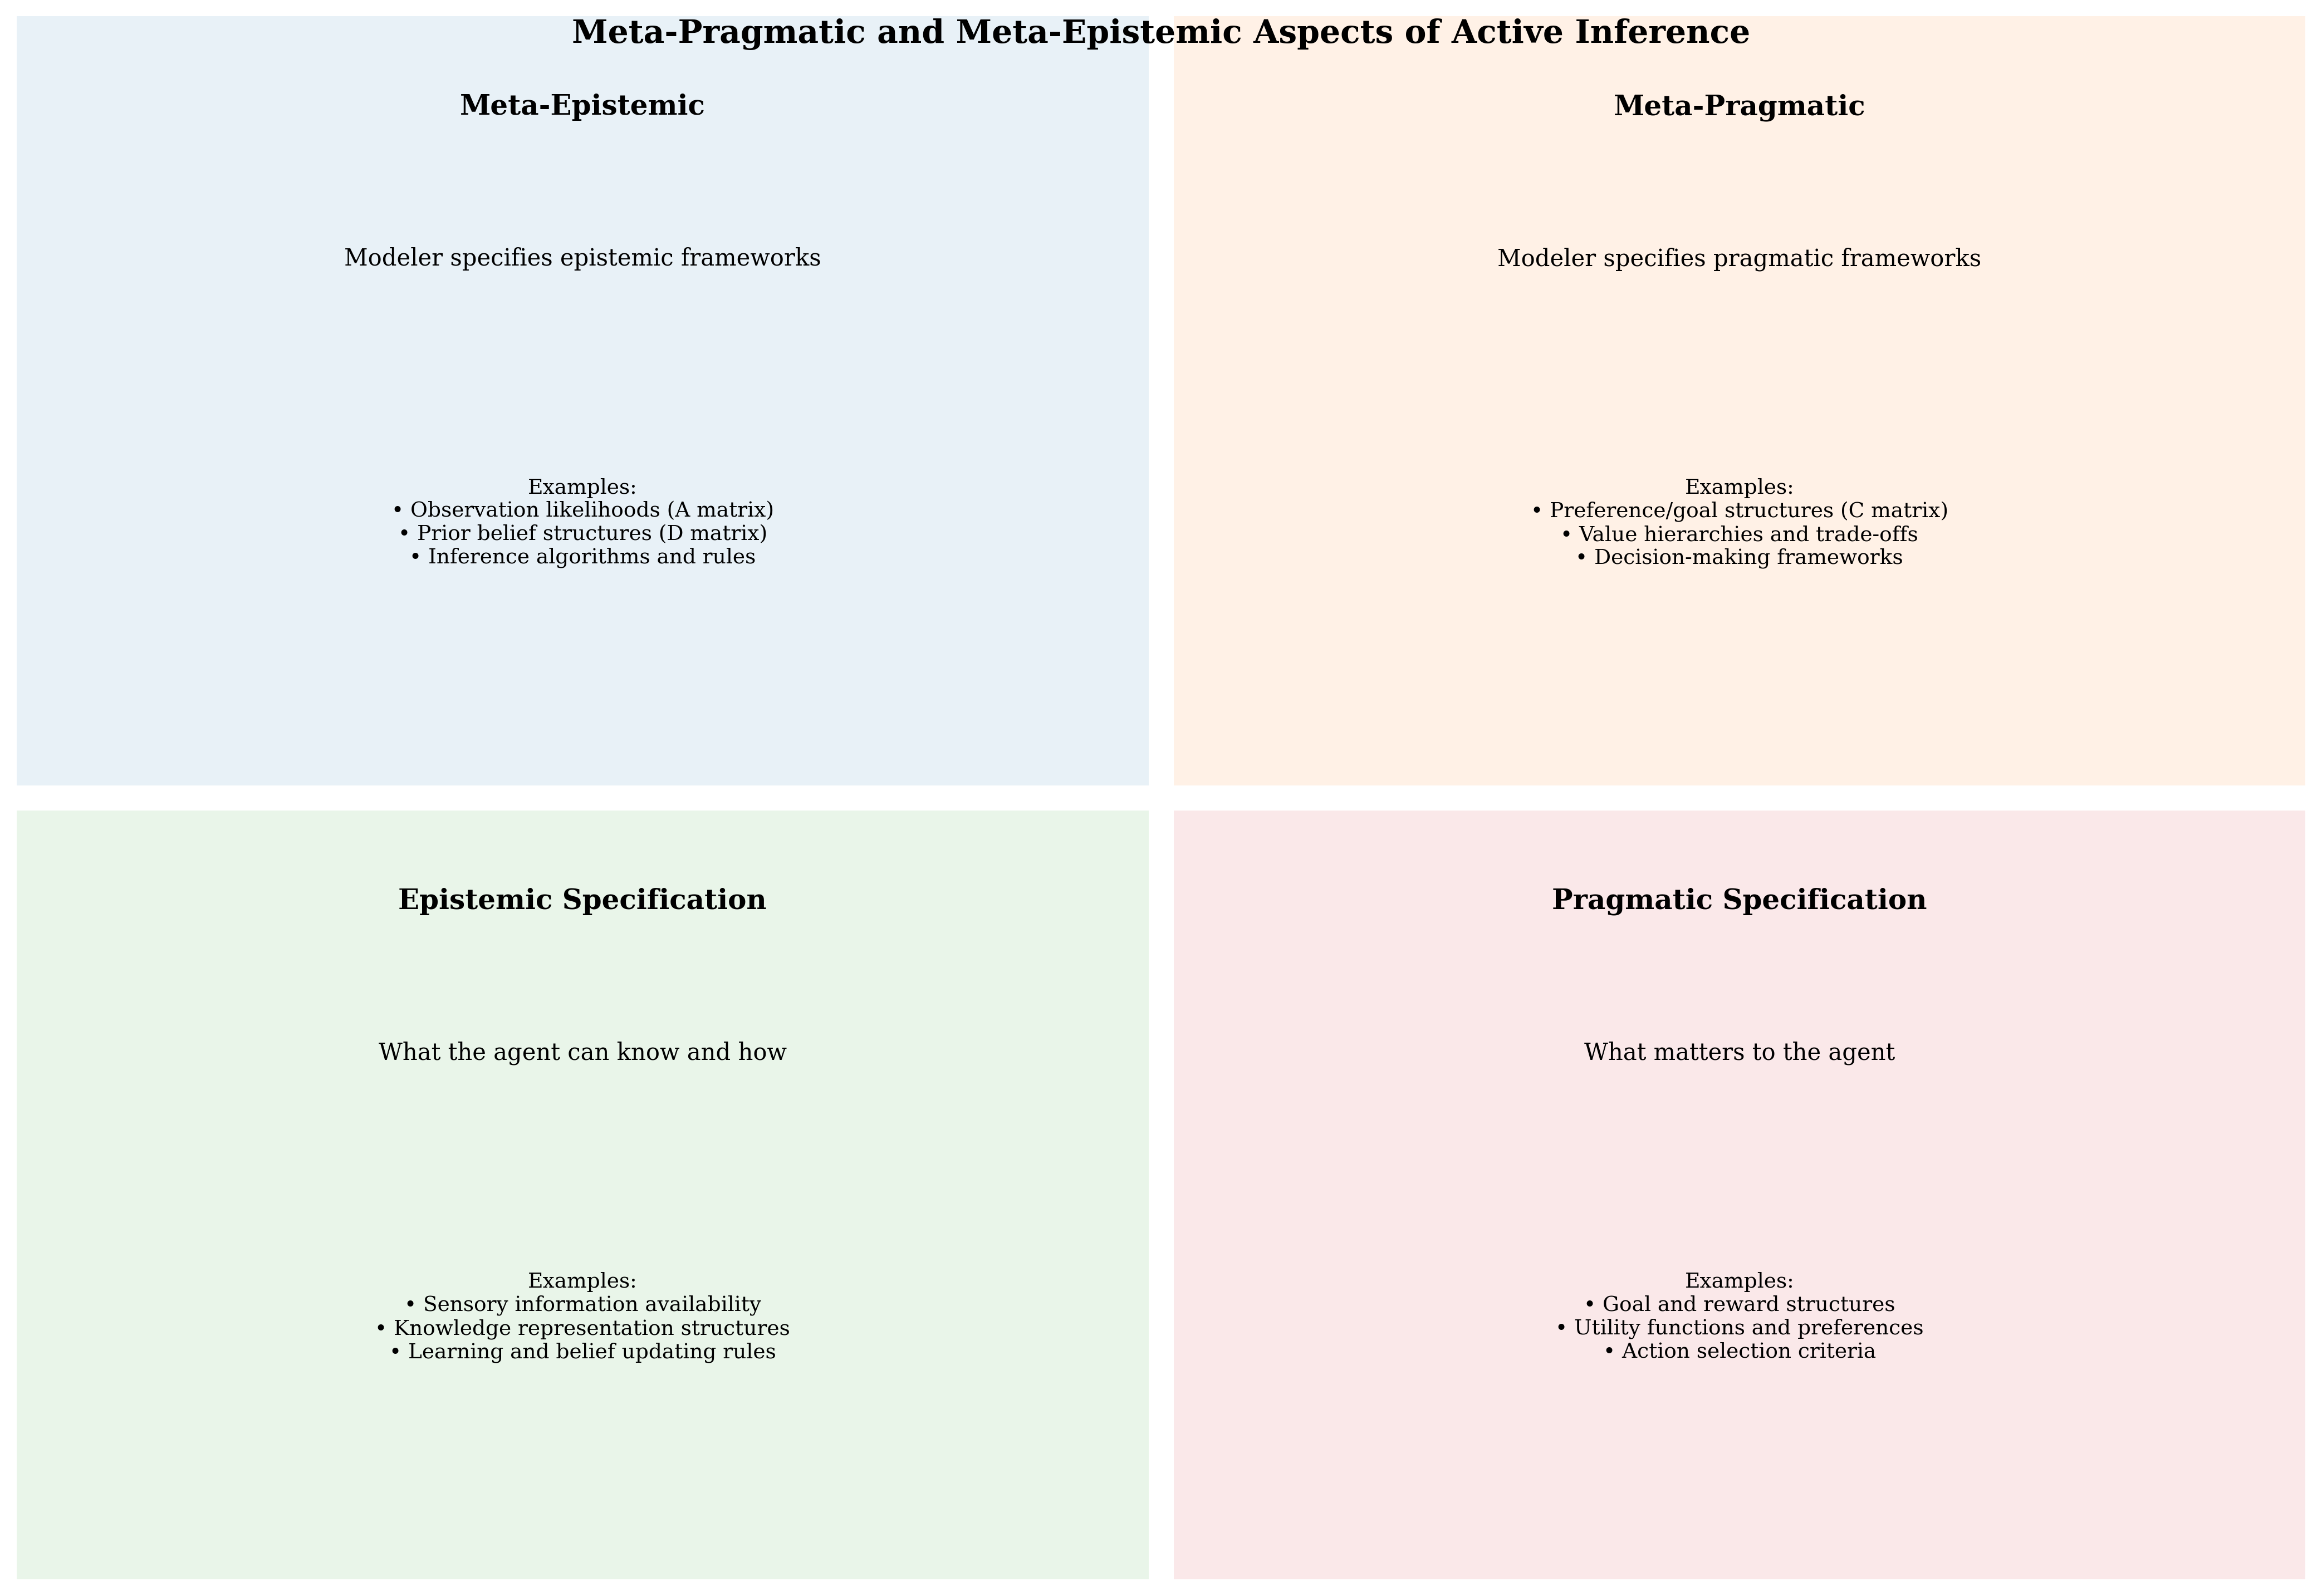
\includegraphics[width=0.8\textwidth]{../figures/meta_level_concepts.png}
\caption{Meta-cognitive processing architecture showing the hierarchical relationship between cognitive and meta-cognitive levels. Meta-cognition monitors and regulates lower-level cognitive processes, enabling self-reflection, confidence assessment, and adaptive strategy selection. In the context of cognitive security, each meta-cognitive level represents both a potential vulnerability (if compromised) and a defensive capability (if properly secured). Higher-order meta-cognition (Quadrant 4) can detect attacks on lower levels.}
\label{fig:meta_cognition_diagram}
\end{figure}

\begin{block}{Attack Surface by Quadrant}
\protect\phantomsection\label{attack-surface-by-quadrant}
{\def\LTcaptype{none} % do not increment counter
\begin{longtable}[]{@{}
  >{\raggedright\arraybackslash}p{(\linewidth - 6\tabcolsep) * \real{0.2439}}
  >{\raggedright\arraybackslash}p{(\linewidth - 6\tabcolsep) * \real{0.1951}}
  >{\raggedright\arraybackslash}p{(\linewidth - 6\tabcolsep) * \real{0.3659}}
  >{\raggedright\arraybackslash}p{(\linewidth - 6\tabcolsep) * \real{0.1951}}@{}}
\toprule\noalign{}
\begin{minipage}[b]{\linewidth}\raggedright
Quadrant
\end{minipage} & \begin{minipage}[b]{\linewidth}\raggedright
Target
\end{minipage} & \begin{minipage}[b]{\linewidth}\raggedright
Vulnerability
\end{minipage} & \begin{minipage}[b]{\linewidth}\raggedright
Impact
\end{minipage} \\
\midrule\noalign{}
\endhead
Q1 & Sensory data & Observation manipulation & Belief distortion \\
Q2 & Meta-data & Quality score falsification & Confidence
miscalibration \\
Q3 & Self-monitoring & Confidence mechanism hijacking & Strategy
corruption \\
Q4 & Framework parameters & Epistemic/pragmatic subversion &
Architectural compromise \\
\bottomrule\noalign{}
\end{longtable}
}

Higher quadrants represent more fundamental vulnerabilities: while
Quadrant 1 attacks can distort specific beliefs, Quadrant 4 attacks can
compromise the entire cognitive architecture.
\end{block}
\end{block}

\begin{block}{Meta-Cognitive Vulnerabilities}
\protect\phantomsection\label{sec:vulnerabilities}
\begin{block}{Quadrant 3 Attacks: Confidence Manipulation}
\protect\phantomsection\label{quadrant-3-attacks-confidence-manipulation}
Manipulation of confidence assessment mechanisms can undermine
meta-cognitive control:

\textbf{False Confidence Calibration:} Adversaries provide feedback that
systematically miscalibrates confidence assessments, causing agents to
over-trust or under-trust their inferences.

\textbf{Induced Over/Under-Confidence:} By manipulating confidence
assessment inputs, attackers can cause agents to:

\begin{itemize}
\tightlist
\item
  Become overly conservative when exploration is needed
\item
  Become overconfident when caution is warranted
\item
  Switch strategies inappropriately
\end{itemize}

\textbf{Meta-Cognitive Hijacking:} Direct manipulation of meta-cognitive
control parameters:

\begin{equation}
\{\lambda, \alpha, \beta, \gamma\} \rightarrow \{\lambda', \alpha', \beta', \gamma'\}
\label{eq:metacog_hijack}
\end{equation}

Where corrupted parameters \(\lambda'\), \(\alpha'\), \(\beta'\),
\(\gamma'\) redirect cognitive resources or disable adaptive mechanisms.
\end{block}

\begin{block}{Quadrant 4 Attacks: Framework Subversion}
\protect\phantomsection\label{quadrant-4-attacks-framework-subversion}
Framework-level manipulation targets the fundamental cognitive
architecture:

\textbf{Epistemic Framework Subversion:} Altering matrices \(A\), \(B\),
or \(D\) through learning or external influence can fundamentally change
what an agent believes is knowable:

\begin{equation}
A_{true} \rightarrow A_{corrupted}: \text{perception of reality distorted}
\label{eq:epistemic_subversion}
\end{equation}

\textbf{Pragmatic Landscape Alteration:} Modifying matrix \(C\) changes
what the agent values:

\begin{equation}
C_{original} \rightarrow C_{corrupted}: \text{goal structure compromised}
\label{eq:pragmatic_alteration}
\end{equation}

This potentially redirects all goal-directed behavior without the
agent's awareness.

\textbf{Higher-Order Reasoning Corruption:} Manipulating framework
optimization processes (Equation \eqref{eq:framework_optimization}) can
cause agents to evolve toward vulnerable or exploitable cognitive
architectures.
\end{block}

\begin{block}{Attack Vector Analysis}
\protect\phantomsection\label{attack-vector-analysis}
\textbf{Gradual vs.~Sudden Attacks:}

\begin{itemize}
\tightlist
\item
  Gradual: Slow parameter drift below detection threshold
\item
  Sudden: Rapid framework changes triggering immediate adaptation
\end{itemize}

\textbf{External vs.~Internal:}

\begin{itemize}
\tightlist
\item
  External: Environmental manipulation of observations
\item
  Internal: Direct parameter injection through learning mechanisms
\end{itemize}

\textbf{Targeted vs.~Systemic:}

\begin{itemize}
\tightlist
\item
  Targeted: Specific quadrant or parameter manipulation
\item
  Systemic: Cascading attacks affecting multiple levels
\end{itemize}
\end{block}
\end{block}

\begin{block}{Formal Threat Model}
\protect\phantomsection\label{sec:threat_model}
We formalize the cognitive security threat model using the quadrant
structure. Let \(\mathcal{M} = (A, B, C, D)\) denote the complete
generative model and \(\Theta = (\lambda, \alpha, \beta, \gamma)\) the
meta-cognitive parameters. An adversary \(\mathcal{A}\) with access
level \(\ell \in \{1,2,3,4\}\) corresponding to quadrant targets can
execute attacks of the form:

\begin{equation}
\mathcal{A}_\ell: (\mathcal{M}, \Theta) \rightarrow (\mathcal{M}', \Theta') \quad \text{s.t. } \|\mathcal{M}' - \mathcal{M}\| + \|\Theta' - \Theta\| \leq \delta_\ell
\label{eq:threat_model}
\end{equation}

The budget \(\delta_\ell\) constrains attack magnitude, reflecting the
principle that higher-quadrant attacks require greater adversarial
capability but produce more fundamental compromise.

\begin{block}{Threat Severity Hierarchy}
\protect\phantomsection\label{threat-severity-hierarchy}
{\def\LTcaptype{none} % do not increment counter
\begin{longtable}[]{@{}
  >{\centering\arraybackslash}p{(\linewidth - 8\tabcolsep) * \real{0.1190}}
  >{\raggedright\arraybackslash}p{(\linewidth - 8\tabcolsep) * \real{0.1905}}
  >{\raggedright\arraybackslash}p{(\linewidth - 8\tabcolsep) * \real{0.4524}}
  >{\centering\arraybackslash}p{(\linewidth - 8\tabcolsep) * \real{0.1190}}
  >{\centering\arraybackslash}p{(\linewidth - 8\tabcolsep) * \real{0.1190}}@{}}
\toprule\noalign{}
\begin{minipage}[b]{\linewidth}\centering
Access Level
\end{minipage} & \begin{minipage}[b]{\linewidth}\raggedright
Target
\end{minipage} & \begin{minipage}[b]{\linewidth}\raggedright
Required Capability
\end{minipage} & \begin{minipage}[b]{\linewidth}\centering
Detectability
\end{minipage} & \begin{minipage}[b]{\linewidth}\centering
Reversibility
\end{minipage} \\
\midrule\noalign{}
\endhead
\(\ell = 1\) & Observations \(o_t\) & Environmental access & High &
Easy \\
\(\ell = 2\) & Meta-data \(\{c(t), r(t)\}\) & Channel compromise &
Medium & Moderate \\
\(\ell = 3\) & Parameters \(\Theta\) & Model access & Low & Difficult \\
\(\ell = 4\) & Model \(\mathcal{M}\) & Architecture access & Very low &
Very difficult \\
\bottomrule\noalign{}
\end{longtable}
}

This hierarchy reveals an inverse relationship between detectability and
impact: Q1 attacks are easily detected but limited in scope, while Q4
attacks are difficult to detect but can compromise the entire cognitive
architecture.
\end{block}

\begin{block}{Real-World Attack Mapping}
\protect\phantomsection\label{real-world-attack-mapping}
The quadrant threat model maps onto documented information operations
and cognitive manipulation campaigns:

\textbf{Q1---Observation manipulation.} Deepfake media and manipulated
imagery inject false observations into agents' sensory streams. This
corresponds to corrupting the data processed under the \(A\) matrix,
causing posterior beliefs \(q(s)\) to diverge from ground truth.

\textbf{Q2---Meta-data falsification.} Coordinated inauthentic behavior
on social platforms {[}@woolley2016political{]} fabricates engagement
metrics, follower counts, and source credibility signals. These are
meta-data attacks: the underlying content may be accurate, but its
perceived reliability (\(c(t)\), \(r(t)\)) is artificially inflated or
deflated, distorting confidence-weighted inference (Equation
\eqref{eq:confidence_weighted_inference}).

\textbf{Q3---Confidence manipulation.} Information disorder campaigns
{[}@wardle2017information{]} do not merely inject false claims but
systematically undermine confidence in legitimate information sources.
The ``firehose of falsehood'' strategy operates at Q3 by overwhelming
meta-cognitive monitoring: agents cannot calibrate confidence when the
base rate of reliable information drops below the detection threshold
\(\gamma\). This corresponds to hijacking the confidence assessment
function (Equation \eqref{eq:confidence_assessment}).

\textbf{Q4---Framework subversion.} Epistemic tribalism and filter
bubbles {[}@benkler2018network{]} represent Q4 attacks on shared
generative models. When communities adopt incompatible \(A\) matrices
(different mappings from evidence to belief), they construct
incommensurable epistemic frameworks. The ``regimes of expectations''
described by @constant2019regimes show how cultural affordances shape
the very generative models through which agents interpret the world,
making framework-level manipulation a societal-scale threat.
\end{block}

\begin{block}{Cascading Attack Dynamics}
\protect\phantomsection\label{cascading-attack-dynamics}
Quadrant attacks can cascade upward. A sustained Q1 campaign (false
observations) can corrupt Q2 meta-data (eroding confidence calibration),
which in turn destabilizes Q3 monitoring (agents cannot distinguish
reliable from unreliable strategies), ultimately enabling Q4 framework
drift (agents adopt corrupted generative models as normative). This
cascading dynamic explains why information warfare campaigns combine
multiple attack vectors simultaneously rather than targeting a single
processing level.
\end{block}

\begin{block}{Comparison: Active Inference Cognitive Defense
vs.~Traditional Cybersecurity}
\protect\phantomsection\label{comparison-active-inference-cognitive-defense-vs.-traditional-cybersecurity}
The quadrant framework offers a cognitive defense paradigm that extends
beyond the scope of traditional information security:

{\def\LTcaptype{none} % do not increment counter
\begin{longtable}[]{@{}
  >{\raggedright\arraybackslash}p{(\linewidth - 4\tabcolsep) * \real{0.1528}}
  >{\raggedright\arraybackslash}p{(\linewidth - 4\tabcolsep) * \real{0.3611}}
  >{\raggedright\arraybackslash}p{(\linewidth - 4\tabcolsep) * \real{0.4861}}@{}}
\toprule\noalign{}
\begin{minipage}[b]{\linewidth}\raggedright
Dimension
\end{minipage} & \begin{minipage}[b]{\linewidth}\raggedright
Traditional Cybersecurity
\end{minipage} & \begin{minipage}[b]{\linewidth}\raggedright
Active Inference Cognitive Defense
\end{minipage} \\
\midrule\noalign{}
\endhead
\textbf{Threat model} & Technical exploits, unauthorized access &
Cognitive manipulation, belief distortion, value corruption \\
\textbf{Attack surface} & Network perimeters, software vulnerabilities &
Information channels (Q1), meta-data streams (Q2), confidence mechanisms
(Q3), framework parameters (Q4) \\
\textbf{Defense paradigm} & Perimeter security, access control &
Multi-level cognitive monitoring across all four quadrants \\
\textbf{Detection method} & Signature matching, behavioral anomaly
detection & Confidence calibration (Q3), framework integrity checking
(Q4), recursive validation \\
\textbf{Protected assets} & Data confidentiality, integrity,
availability & Epistemic autonomy (\(A\), \(B\), \(D\)), pragmatic
autonomy (\(C\)), framework coherence (\(\Theta\)) \\
\textbf{Adaptation} & Patch management, rule updates & Self-monitoring
(Q3), framework evolution (Q4) \\
\textbf{Scope} & Individual systems, networks & Individual cognition,
collective sense-making, institutional epistemics \\
\bottomrule\noalign{}
\end{longtable}
}

The key advantage of the Active Inference approach is its capacity for
\emph{recursive self-defense}: meta-cognitive monitoring (Q3) can detect
attacks on lower quadrants, while framework integrity checking (Q4) can
detect attacks on meta-cognitive mechanisms themselves. This recursive
property has no direct analogue in traditional cybersecurity, which
relies on external monitoring rather than self-reflective integrity
verification.
\end{block}
\end{block}

\begin{block}{Defense Strategies}
\protect\phantomsection\label{sec:defense_strategies}
The framework suggests defense approaches operating at multiple levels,
with higher-level defenses providing more fundamental protection.

\begin{block}{Meta-Cognitive Monitoring (Quadrant 3 Defense)}
\protect\phantomsection\label{meta-cognitive-monitoring-quadrant-3-defense}
Continuous validation of confidence assessments:

\begin{equation}
validation(c) = |accuracy_{predicted}(c) - accuracy_{actual}|
\label{eq:confidence_validation}
\end{equation}

\textbf{Defense Mechanisms:}

\begin{itemize}
\tightlist
\item
  Cross-validation of confidence with actual performance
\item
  Detection of miscalibration patterns
\item
  Anomaly detection for confidence trajectories
\item
  Automatic recalibration when drift detected
\end{itemize}
\end{block}

\begin{block}{Framework Integrity Checks (Quadrant 4 Defense)}
\protect\phantomsection\label{framework-integrity-checks-quadrant-4-defense}
Verification of epistemic and pragmatic consistency:

\begin{equation}
integrity(\Theta) = \|\Theta_t - \Theta_{baseline}\| < \epsilon
\label{eq:framework_integrity}
\end{equation}

\textbf{Defense Mechanisms:}

\begin{itemize}
\tightlist
\item
  Monitoring framework parameters for unexpected changes
\item
  Detecting drift in matrices \(A\), \(B\), \(C\), \(D\)
\item
  Regularization terms \(\mathcal{R}(\Theta)\) penalizing inconsistent
  specifications
\item
  Framework coherence validation
\end{itemize}
\end{block}

\begin{block}{Recursive Validation (Multi-Level Defense)}
\protect\phantomsection\label{recursive-validation-multi-level-defense}
Higher-order checking of meta-level processes:

\textbf{Three-Layer Validation:}

\begin{enumerate}
\tightlist
\item
  \textbf{Level 1:} Validate primary inference processes
\item
  \textbf{Level 2:} Validate meta-cognitive monitoring itself
\item
  \textbf{Level 3:} Validate framework integrity checking
\end{enumerate}

This recursive structure ensures that each security layer is itself
protected by higher layers.
\end{block}

\begin{block}{Defense Portfolio}
\protect\phantomsection\label{defense-portfolio}
{\def\LTcaptype{none} % do not increment counter
\begin{longtable}[]{@{}lll@{}}
\toprule\noalign{}
Defense Layer & Mechanism & Protects Against \\
\midrule\noalign{}
\endhead
Observation validation & Signal integrity & Q1 attacks \\
Meta-data verification & Source authentication & Q2 attacks \\
Confidence monitoring & Calibration checking & Q3 attacks \\
Framework integrity & Parameter bounds & Q4 attacks \\
Recursive validation & Self-checking & Multi-level attacks \\
\bottomrule\noalign{}
\end{longtable}
}
\end{block}
\end{block}

\begin{block}{AI Safety and Value Alignment}
\protect\phantomsection\label{sec:ai_safety}
The framework provides principled approaches to AI safety challenges
that address concrete problems identified in the alignment literature
{[}@amodei2016concrete; @russell2019human; @gabriel2020artificial{]}.

\begin{block}{Value Specification through Matrix C}
\protect\phantomsection\label{value-specification-through-matrix-c}
Active Inference enables precise value specification through the
preference prior \(C\), offering a structured alternative to scalar
reward functions {[}@ngo2022alignment{]}:

\begin{equation}
C_{safe} = \text{specification of safe preferences}
\label{eq:safe_preferences}
\end{equation}

\textbf{Advantages over reward functions} {[}@russell2019human{]}:

\begin{itemize}
\tightlist
\item
  Multi-dimensional preference landscapes rather than scalar rewards
\item
  Trade-off specification between competing values (safety
  vs.~capability)
\item
  Ethical considerations directly encoded in the generative model
\item
  Value hierarchies with priority structures inspectable by designers
\end{itemize}
\end{block}

\begin{block}{Epistemic Boundary Protection}
\protect\phantomsection\label{epistemic-boundary-protection}
Clear limits on what AI systems can know and assume:

\textbf{Bounded Epistemic Frameworks:}

\begin{itemize}
\tightlist
\item
  Matrix \(A\) specifications limit observation reliability assumptions
\item
  Matrix \(D\) priors constrain initial state assumptions
\item
  Matrix \(B\) causal models bound action effect assumptions
\end{itemize}
\end{block}

\begin{block}{Framework Integrity for AI Systems}
\protect\phantomsection\label{framework-integrity-for-ai-systems}
Protection against value drift and epistemic corruption is essential for
advanced AI systems, where unconstrained framework optimization could
lead to instrumental convergence on undesirable goals
{[}@bostrom2014superintelligence{]}:

\textbf{Meta-Monitoring Requirements:}

\begin{itemize}
\tightlist
\item
  Self-watchful AI systems monitoring their own frameworks via Q3
  confidence validation
\item
  Anomaly detection for framework parameter changes using integrity
  checks (Equation \eqref{eq:framework_integrity})
\item
  Rollback capabilities for detected corruption of \(A\), \(B\), \(C\),
  \(D\) matrices
\item
  Human-in-the-loop for framework modifications at Q4 level
\end{itemize}
\end{block}

\begin{block}{Alignment through Framework Specification}
\protect\phantomsection\label{alignment-through-framework-specification}
The meta-pragmatic aspect enables principled alignment:

\begin{enumerate}
\tightlist
\item
  \textbf{Value Learning:} Systems develop value structures through
  matrix \(C\) optimization
\item
  \textbf{Epistemic Constraints:} Matrix \(A\), \(B\), \(D\)
  specifications limit inference scope
\item
  \textbf{Meta-Cognitive Oversight:} Quadrant 3 monitoring ensures
  alignment maintenance
\item
  \textbf{Framework Stability:} Quadrant 4 regularization prevents
  unauthorized evolution
\end{enumerate}
\end{block}
\end{block}

\begin{block}{Societal Implications}
\protect\phantomsection\label{sec:societal_security}
\begin{block}{Information Warfare}
\protect\phantomsection\label{information-warfare}
The framework reveals meta-level manipulation of public belief systems:

\textbf{Epistemic Attacks on Societies:}

\begin{itemize}
\tightlist
\item
  Systematic manipulation of information quality (meta-data)
\item
  Undermining confidence in legitimate information sources
\item
  Framework-level attacks on shared epistemological foundations
\end{itemize}

\textbf{Defense Implications:}

\begin{itemize}
\tightlist
\item
  Education in meta-cognitive awareness
\item
  Institutional meta-data verification
\item
  Collective framework integrity monitoring
\end{itemize}
\end{block}

\begin{block}{Educational System Resilience}
\protect\phantomsection\label{educational-system-resilience}
Development of curricula building meta-cognitive resilience:

\textbf{Training Quadrant 3 Skills:}

\begin{itemize}
\tightlist
\item
  Self-monitoring and confidence assessment
\item
  Strategy adaptation under uncertainty
\item
  Meta-cognitive awareness
\end{itemize}

\textbf{Training Quadrant 4 Skills:}

\begin{itemize}
\tightlist
\item
  Framework evaluation and critique
\item
  Epistemic framework comparison
\item
  Value system analysis
\end{itemize}
\end{block}

\begin{block}{Collective Cognitive Security}
\protect\phantomsection\label{collective-cognitive-security}
Protection of group-level cognitive processes:

\textbf{Shared Framework Protection:}

\begin{itemize}
\tightlist
\item
  Collective monitoring of epistemic drift
\item
  Group-level confidence calibration
\item
  Democratic framework governance
\end{itemize}

\textbf{Institutional Safeguards:}

\begin{itemize}
\tightlist
\item
  Verification of information sources
\item
  Meta-data authenticity standards
\item
  Framework change transparency
\end{itemize}
\end{block}
\end{block}

\begin{block}{Ethical Considerations}
\protect\phantomsection\label{sec:security_ethics}
\begin{block}{Manipulation Risks}
\protect\phantomsection\label{manipulation-risks}
Meta-level cognition raises concerns that extend the problem of
faultless responsibility in distributed systems
{[}@floridi2016faultless{]}:

\begin{itemize}
\tightlist
\item
  Potential for sophisticated cognitive manipulation targeting any
  quadrant
\item
  Exploitation of framework vulnerabilities by actors with asymmetric
  knowledge
\item
  Dual-use nature of meta-cognitive insights: defense tools can also
  inform attacks
\end{itemize}
\end{block}

\begin{block}{Responsibility in Framework Design}
\protect\phantomsection\label{responsibility-in-framework-design}
Designers of cognitive systems bear responsibility for
{[}@floridi2016faultless; @gabriel2020artificial{]}:

\begin{itemize}
\tightlist
\item
  Secure framework specifications with built-in integrity constraints
\item
  Robust defense mechanisms operating at all four quadrant levels
\item
  Transparent vulnerability disclosure and responsible research
  practices
\end{itemize}
\end{block}

\begin{block}{Self-Determination}
\protect\phantomsection\label{self-determination}
Protection of individual and collective:

\begin{itemize}
\tightlist
\item
  Epistemic autonomy: freedom to form beliefs
\item
  Pragmatic autonomy: freedom to set values
\item
  Meta-cognitive autonomy: freedom to adapt frameworks
\end{itemize}
\end{block}
\end{block}
\end{frame}

\end{document}
